\documentclass[../main]{subfiles}

\begin{document}

\section{Atomic Structure}

	\subsection{Structure of the Atom}

	Atoms are made of the nucleus (diameter \SI{10e-14}{\m}) which contains its protons and neutrons and the electron cloud  (diameter \SI{10e-10}{\m}surrounding the nucleus.

	\subsubsection{Deflection in an Electric Field}

	When a beam of particles are passed between two charged electric plates, charged particles experience an electric force which deflects them from the original direction of motion. Negatively charged particles are attracted to positive plates and positively charged particles are attracted to negatively charged plates. The magnitude of deflection or angle of deflection is observed to be proportional to the \(\frac{\text{charge}}{\text{mass}}\) ratio. The larger the charge on a particle the larger the electric force experienced, and the larger the mass the lesser the amount of deviation which results from the same amount of force.

	\subsubsection{Orbitals}

	Electrons do not occupy fixed positions around a nucleus but rather are constantly present in regions of space around the nucleus known as atomic orbitals and have differing levels of energy.

	\scidef{Shell}{A electronic shell is a collection of electrons which share a similar energy level.}

	\scidef{Principal Quantum Number}{The Principal Quantum Number (written as \textbf{n}) is a description of which shell an electron is in. Large values of n imply that the electron tends to move far away from the nucleus as well as having a larger sized orbital (AKA more diffuse), has a high amount of energy and has weaker electrostatic attraction between nucleus and electron.}

	\scidef{Atomic Orbital}{An Atomic Orbital is a certain space around a nucleus where electrons tend to move inside, and where there is a high probability of observing an electron inside. Each atomic orbital has a certain geometry and a certain amount of energy which is described by its principal quantum number. Each orbital can contain a maximum of two electrons.}

	\scidef{Subshell}{Shells are categorized into Subshells which then comprise of electrons with similar geometries. Subshells include the s, p, d and f shells.}

	s orbitals have a spherical shape. s subshells have 1 orbital and contain 2 electrons.\\

	p orbitals have a dumbbell shape which are oriented along perpendicular axis, and are labeled as the \usub{p}{x}, \usub{p}{y} and \usub{p}{z} orbitals. p subshells have 3 orbitals and contain 6 electrons. \\

	d orbitals generally have a 4-lobed shape with three orbitals (\usub{d}{xy}, \usub{d}{xz} and \usub{d}{yz}) pointing between axis, one orbital \usub{d}{\usup{x}{2}-\usup{y}{2}} and one orbital along the z axis as well as a torus along the x-y plane \usub{d}{\usup{z}{2}}. d subshells have 5 orbitals and contain 10 electrons. \\

	The \usup{n}{th} shell will hence have n subshells and contain \usup{n}{2} orbitals and \usup{2n}{2} electrons.

	\subsubsection{Electronic Configuration}

	\scidef{Electronic Configuration}{The Electronic Configuration of a atom or ion is a description of how its electrons are distributed among its shells, subshells and orbitals.}

	\scidef{Isoelectronic Species}{Isoelectronic Species are atoms or ions which have the same number of electrons, regardless of electronic configuration.}

	\scidef{Aufbau Principle}{The Aufbau Principle states that electrons fill the orbitals with the lowest energy level first. The energy level of an orbital is determined by experimentation and has been estimated by equations such as the Schr\"{o}dinger equation.

		\begin{center} 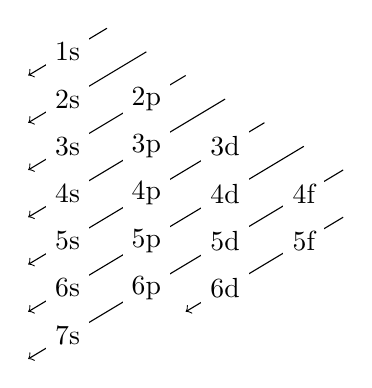
\begin{tikzpicture}
			\draw[->] (1,-0.3) -- (0,-0.9);
			\draw[->] (1.5,-0.6) -- (0,-1.5);
			\draw[->] (2,-0.9) -- (0,-2.1);
			\draw[->] (2.5,-1.2) -- (0,-2.7);
			\draw[->] (3,-1.5) -- (0,-3.3);
			\draw[->] (3.5,-1.8) -- (0,-3.9);
			\draw[->] (4,-2.1) -- (0,-4.5);
			\draw[->] (4,-2.7) -- (2,-3.9);
			\foreach \s in {1,2,3,4,5,6,7}
    			\draw (0.5, {-\s*0.6} ) node[fill=white] {\s s};
    		\foreach \p	in {2,3,4,5,6}
    			\draw (1.5, {-\p*0.6} ) node[fill=white] {\p p};
    		\foreach \d	in {3,4,5,6}
    			\draw (2.5, {-\d*0.6} ) node[fill=white] {\d d};
    		\foreach \f	in {4,5}
    			\draw (3.5, {-\f*0.6} ) node[fill=white] {\f f};
		\end{tikzpicture} \end{center}

		Note that the 4s orbital fills before the 3d orbital.
	}

	\scidef{Pauli Exclusion Principle}{The Pauli Exclusion Principle states that one orbital can contain a maximum of two electrons and that they must be of opposite spins in order to reduce intra-electronic repulsion through magnetic attraction as a result of their opposite spin.}

	\scidef{Hund's Rule}{Hund's Rule states that orbitals in a subshell must all have at least one electron before any orbital can have two in order to minimise intra-electronic repulsion.}

	Exceptions governing electronic configuration:\\

	\begin{description}
		\item[Group 6] elements have electronic configuration of \usup{d}{5} \usup{s}{1} rather than  \usup{d}{4} \usup{s}{2} since inter-electronic repulsion is minimized. \usup{d}{4} shells are generally not observed. One example of such an element is Cr with configuration [Ar] \usup{3d}{5} \usup{4s}{1}
		\item[Group 11] elements have electronic configuration of \usup{d}{10} \usup{s}{1} rather than \usup{d}{9} \usup{s}{2} since a fully filled d subshell is more stable than the 4s subshell due to geometric symmetry. \usup{d}{9} shells are generally not observed. One example of such an element is Cu with configuration [Ar] \usup{3d}{10} \usup{4s}{1}
	\end{description}

	\subsubsection{Written Electronic Configuration}

	Electronic configuration is written as a series of subshells and the amount of electrons present in the orbital. \\

	Electronic Configuration for Xenon: \usup{1s}{2} \usup{2s}{2} \usup{2p}{6} \usup{3s}{2} \usup{3p}{6} \usup{4s}{2} \usup{4p}{6} \usup{4d}{10} \usup{5s}{2} \usup{5d}{10} 

	In long answer questions, when explaining electronic configuration, shorthand can be used. \\

	Electronic Configuration for Cesium: [Xe] \usup{6s}{1} \\

	\subsubsection{Energy Level Diagrams}

	Energy level diagrams are used to represent the energy levels of differing orbitals. The y axis is labeled as energy while to the right each subshell's orbitals are represented as a dash, with electrons in an orbital represented as arrows. 

		\begin{center} 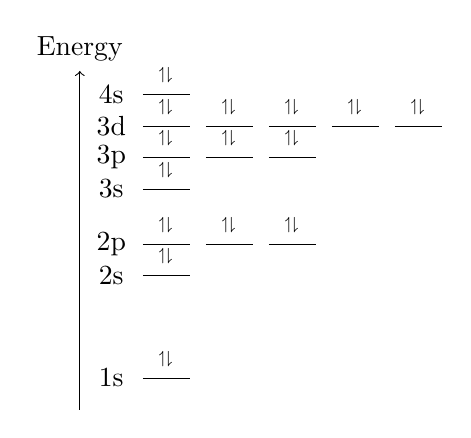
\begin{tikzpicture}

		\draw[->] (0,0) -- (0,4.3) node[anchor=south] {Energy};

		\draw (0.4,0.4) node {1s};
		\foreach \x in {1}
			\draw ({\x*0.8},0.4) -- ({\x*0.8+0.6},0.4) node[midway,anchor=south] {
				\tiny \rotatebox{90}{\(\rightharpoonup\)}\rotatebox{90}{\(\leftharpoondown\)}};

		\draw (0.4,1.7) node {2s};
		\foreach \x in {1}
			\draw ({\x*0.8},1.7) -- ({\x*0.8+0.6},1.7) node[midway,anchor=south] {
				\tiny \rotatebox{90}{\(\rightharpoonup\)}\rotatebox{90}{\(\leftharpoondown\)}};

		\draw (0.4,2.1) node {2p};
		\foreach \x in {1,2,3}
			\draw ({\x*0.8},2.1) -- ({\x*0.8+0.6},2.1) node[midway,anchor=south] {
				\tiny \rotatebox{90}{\(\rightharpoonup\)}\rotatebox{90}{\(\leftharpoondown\)}};

		\draw (0.4,2.8) node {3s};
		\foreach \x in {1}
			\draw ({\x*0.8},2.8) -- ({\x*0.8+0.6},2.8) node[midway,anchor=south] {
				\tiny \rotatebox{90}{\(\rightharpoonup\)}\rotatebox{90}{\(\leftharpoondown\)}};

		\draw (0.4,3.2) node {3p};
		\foreach \x in {1,2,3}
			\draw ({\x*0.8},3.2) -- ({\x*0.8+0.6},3.2) node[midway,anchor=south] {
				\tiny \rotatebox{90}{\(\rightharpoonup\)}\rotatebox{90}{\(\leftharpoondown\)}};

		\draw (0.4,3.6) node {3d};
		\foreach \x in {1,2,3,4,5}
			\draw ({\x*0.8},3.6) -- ({\x*0.8+0.6},3.6) node[midway,anchor=south] {
				\tiny \rotatebox{90}{\(\rightharpoonup\)}\rotatebox{90}{\(\leftharpoondown\)}};

		\draw (0.4,4) node {4s};
		\foreach \x in {1}
			\draw ({\x*0.8},4) -- ({\x*0.8+0.6},4) node[midway,anchor=south] {
				\tiny \rotatebox{90}{\(\rightharpoonup\)}\rotatebox{90}{\(\leftharpoondown\)}};

		\end{tikzpicture} \end{center}


	\subsubsection{Electronic Configuration of Ions}

	Anions have electrons added to the next energetically accessible orbital. Electronic configuration is calculated as usual. \\

	Cations have their electrons removed from the orbital of highest energy. Electrons occupy the orbital of lowest energy level first (4s before 3d), but once inner orbitals are filled these inner orbitals will repel outermost orbitals and promote them to a higher energy level (hence 4s is removed before 3d when being ionized). \\

	Keep in mind that electronically accessible \(\neq\) highest/lowest energy.

	\subsubsection{Excited Particles}

	\scidef{Ground State}{An atom or ion is in its ground state when all electrons are in orbitals of the lowest available energy level / at its most stable.}

	\scidef{Excited State}{An atom or ion in an excited state has absorbed energy and has electrons which are promoted to higher energy levels, which can then emit energy to return to ground state. Excited particles are denoted with an asterisk to the right (C*).}

	\subsection{Periodic Table Trends}

	\subsubsection{Common Properties}

	There are three main factors which affect properties of atoms:

	\begin{description}
	\item[Number of Electronic Shells]:\\
		The higher the principal quantum number of an atom, the larger the distance between the nucleus and its valence electrons and hence the weaker the electrostatic attraction between the nucleus and the valence electrons.
	\item[Size of Nuclear Charge]:\\
		The larger the number of protons in an atom, the stronger the electrostatic attraction between the nucleus and the valence electrons.
	\item[Shielding Effect by Inner Electrons]:\\
		The larger the number of inner shell electrons, the larger the shielding effect experienced by the valence electrons and hence the weaker the electrostatic attraction between the nucleus and the valence electrons. \\
		All electrons repel each other due to their negative charge, hence electrons in inner shells repel electrons in outer shells and prevent outer electrons from experiencing the full nuclear charge.
	\end{description}

	\scidef{Effective Nuclear Charge}{The Effective Nuclear Charge is the combination of the effects of size of nuclear charge with shielding effect by inner electrons on the strength of electrostatic attraction between nucleus and valence electrons of a particle, typically used when comparing elements down a period.}

	Explanations tend to follow a pattern of [Down a group / Across a period] \(\rightarrow\) [\# of shells + Nuclear Charge + Shielding] \(\rightarrow\) [Electrostatic Attraction increases/decreases] \(\rightarrow\) [Property].\\

	Across a period:
	\begin{description}
		\item[Number of Electronic Shells] remains constant.
		\item[Effective Nuclear Charge] increases as number of protons increases to increase the nuclear charge and though the number of electrons increase, they are added to the same quantum shell which means shielding effect remains approximately constant.
		\item[Electrostatic Attraction] between nucleus and valence electrons hence increases across a period.
	\end{description}

	Down a group:
	\begin{description}
		\item[Number of Electronic Shells] increases, increasing the distance between valence electrons and the nucleus.
		\item[Nuclear Charge] may increase, but is not as significant.
		\item[Electrostatic Attraction] between nucleus and valence electrons hence decreases down a group.
	\end{description}

	\subsubsection{Electronegativity}

	\scidef{Electronegativity}{Electronegativity is the tendency of an atom to attract bonding electrons.}

	Electronegativity increases as electrostatic attraction increases.

	\subsubsection{Atomic Radius}

	\scidef{Atomic Radius}{Atomic Radius is the shortest inter-nuclear distance found in the structure of an element. Metallic elements calculate radius from half the distance between to neighboring atoms in a metal. Covalent elements calculate radius from half the distance between two bonded atoms. Monatomic elements calculate radius from half the distance between two atoms which are not bonded.}

	Atomic radius increases as electrostatic attraction decreases.

	\subsubsection{Ionic Radius}

	\scidef{Ionic Radius}{Ionic Radius is the radius of the spherical ion in an ionic compound.}

	Ionic Radius of isoelectronic species increase as electrostatic attraction decreases.

	\subsubsection{First Ionization Energy}

	\scidef{First Ionization Energy}{The First Ionization Energy of a atom is the amount of energy required to be supplied to remove one mole of \ch{e-} from one mole of gaseous atoms.}

	First Ionization Energy increases as electrostatic attraction increases. \\

	Two exceptions occur to this trend:

	\begin{description}
		\item[Group 2 and 13] notices that group 13 elements have a lower first IE than group 2 elements, since the p electron in group 13 is at a higher energy level than that of the s electron in a group 2, hence less energy is needed to remove electrons from the group 13 element.
		\item[Group 15 and 16] notices that group 16 elements have a lower first IE than group 15 elements since the paired p orbital in group 16 elements exhibits inter-electronic repulsion that is not present in the group 15 element with unpaired p orbitals, hence less energy is required to remove electrons from the group 16 element.
	\end{description}

	\subsubsection{nth Ionization Energy}

	Successive IEs of an element increase since each successive electron being removed is being extracted from an ion of increasing positive charge which attracts its electrons more strongly. \\

	There is a large increase of IE when electrons are removed from a different quantum shell and a smaller increase of IE when electrons are removed from a different subshell. Use these observations to infer the group of an element when given its successive IEs. \\

\end{document}